\documentclass[11pt,a4paper]{article}

% ---------------------------------------------------------------------------
% Reliable autocatalytic operation with a finite fuel-waste bath.
%
% Author metadata: set the macros below before submission.  They are
% deliberately left blank in this version.  \CompanionAuthor is the author
% printed for the companion manuscripts in refs.bib; \RepositoryNote is where
% the public repository location goes.
% ---------------------------------------------------------------------------
\newcommand{\PaperAuthor}{}
\newcommand{\PaperAffiliation}{}
\newcommand{\PaperDate}{19 September 2026}
\newcommand{\CompanionAuthor}{Anonymous}
\newcommand{\RepositoryNote}{The repository location will be supplied with the author information.}

\usepackage[T1]{fontenc}
\usepackage[utf8]{inputenc}
\usepackage{lmodern}
\usepackage{microtype}
\usepackage[a4paper,margin=1.05in]{geometry}
\usepackage{amsmath,amssymb,amsthm,mathtools}
\usepackage{booktabs}
\usepackage{array}
\usepackage{longtable}
\usepackage{enumitem}
\usepackage{xcolor}
\usepackage{graphicx}
\usepackage{capt-of}
\usepackage{tikz}
\usetikzlibrary{arrows.meta,positioning,calc}
\usepackage[obeyspaces,spaces]{url}
\usepackage[numbers,sort&compress]{natbib}
\usepackage[colorlinks=true,linkcolor=blue!55!black,citecolor=blue!55!black,urlcolor=blue!55!black]{hyperref}
\hypersetup{pdftitle={Reliable autocatalytic operation with a finite fuel-waste bath},
  pdfkeywords={autocatalysis, finite reservoirs, stochastic reaction networks, local detailed balance, uniformization, exponential martingales, reservoir sizing, Lean}}

\DeclareUrlCommand\lean{\urlstyle{tt}}
\setlist{itemsep=2pt,topsep=3pt}
\setlength{\emergencystretch}{1.5em}
\graphicspath{{figures/}}

\theoremstyle{plain}
\newtheorem{theorem}{Theorem}[section]
\newtheorem{proposition}[theorem]{Proposition}
\newtheorem{lemma}[theorem]{Lemma}
\newtheorem{corollary}[theorem]{Corollary}
\theoremstyle{definition}
\newtheorem{definition}[theorem]{Definition}
\theoremstyle{remark}
\newtheorem{remark}[theorem]{Remark}

\newcommand{\R}{\mathbb R}
\newcommand{\N}{\mathbb N}
\newcommand{\Z}{\mathbb Z}
\newcommand{\Prob}{\mathbb P}
\newcommand{\E}{\mathbb E}
\newcommand{\eps}{\varepsilon}
\newcommand{\cR}{\mathcal R}
\newcommand{\Lgen}{\mathcal L}
\newcommand{\Iv}{I}
\newcommand{\Pnet}{P_{\mathrm{net}}}
\newcommand{\one}{\mathbf 1}

\title{Reliable autocatalytic operation with a\\ finite fuel--waste bath:\\[4pt]
\large joint mission guarantees, reservoir sizing and a sharpened certificate}
\author{\PaperAuthor\\ \small \PaperAffiliation}
\date{\PaperDate}

\begin{document}
\maketitle

\begin{abstract}
A reactor that is repeatedly thinned, refed and harvested must recover its catalytic stock, deliver product, and leave a state from which the next operation can succeed. If its fuel is a genuinely finite molecular inventory rather than a chemostatted activity, then every driven event also changes the chemistry of the next operation, and the guarantee has to be proved for that changed stochastic law. We prove a joint finite-horizon operating theorem for an explicitly specified six-species count reactor coupled to a conserved two-species fuel/waste bath of total inventory $M$ and reference capacity $R$, in which the driven channel $X+F\rightleftharpoons U+W+P$ moves one molecule between the two bath species at every event and its two directed propensities are proportional to the current bath fractions $f/R$ and $p/R$. One event on the full normalized history law requires, in every one of $m$ externally clocked cycles, return of the actual endpoint to an explicit restart set, two overlapping collected-output thresholds, two food allowances and a gross driven-service allowance, together with an all-prefix bound on the bath composition and a pathwise net-synthesis statement for every physical realization. For every admitted bath state, every parameter in the class $19\le r\le21$, $d\ge0$, $dM\le R/25$ and every controller acting on the returned history, the probability that all $m$ cycles succeed is at least $(1-e(V))^{m}\ge1-m\,e(V)$.

We then sharpen the certificate in two independent ways and propagate both through the entire chain. First, the published phase-transport exponent discards a factor: the unrounded rate is $\kappa=1839/(8.75\times10^{12})=2.1017\ldots\times10^{-10}$ rather than $10^{-10}$, and a new absorption estimate makes $e(V)\le101e^{-\kappa V}$ valid from $V\ge10^{10}$ instead of $2\times10^{11}$. Second, on the pure-fuel bath at $d=1/50$ the two directed service intensities are controlled by \emph{correlated} bath fractions summing to one, which halves the certified per-cycle gross allowance from $\lfloor V/5\rfloor$ to $\lfloor V/10\rfloor$ inside the same error budget, and therefore halves the sufficient reservoir at fixed copy scale. Together they give the design rule $V=\max\bigl(5\times10^{10},\lceil\kappa^{-1}\log(101m/\delta)\rceil,\lceil56D_I/m\rceil,\lceil1080D_X/m\rceil\bigr)$, $R=\max(1,\lceil m\lfloor V/10\rfloor/\rho\rceil)$. The hundred-cycle instance certified at $V=2\times10^{11}$, $R=4\times10^{13}$ with confidence $99.9979\%$ is matched at $V=9.6\times10^{10}$, $R=9.6\times10^{12}$; at the original copy scale the same mission now has failure probability at most $10^{-13}$ with half the fuel. We also give exact finite-bath endpoint free energies, a finite metered-food corollary and deterministic diagnostics separating productive output from fuel turnover. The whole chain, including nonexplosion, the identification of the stopped device with the physical process, the repetition argument and both refinements, is verified in Lean~4 with Mathlib; an exact replay script re-derives every printed constant. The reactor is a schematic benchmark with established catalyst and externally implemented feeds and interventions; reliable production does not imply positive net fuel consumption.
\end{abstract}

\section{Introduction}\label{sec:intro}

Structural theories of autocatalysis~\citep{kauffman1986,hordijk2004,steel2019,blokhuis2020} identify which reaction networks can regenerate their catalysts from a food set. The operational test applied in the laboratory is the serial-transfer protocol~\citep{mills1967,lincoln2009,adamski2020,ameta2021}: a fraction of the mixture is diluted into fresh food and the system is called self-sustaining if it regrows far enough for the next transfer to succeed, repeatedly. Companion work made that test quantitative for one explicitly specified, reversible and thermochemically consistent chemistry: first for the mass-action concentration equations~\citep{recovery2026}, then at finite molecule number~\citep{finitecopy2026}, where each cycle is a random thinning of individual molecules followed by four units of a twenty-channel Markov jump process, and $m$ consecutive successes are certified jointly.

All of that assumed maintained fuel and waste: the driven channel ran at activities pinned to one, as in the chemostatted idealization of open-network thermodynamics~\citep{polettini2014,rao2016}. A real driven reaction consumes a finite inventory. The present paper removes that idealization for the same chemistry. The fuel $F$ and waste $P$ become two more counted species with conserved total $f+p=M$, held in a bath of reference capacity $R$ that is neither reset nor replenished between cycles, and the two directed propensities of the driven pair become proportional to the current fractions $f/R$ and $p/R$.

\paragraph{Why this is not a corollary of the maintained-bath theorem.}
Changing the bath changes the generator, so it changes the law of every observable the earlier proof controls. The reactor's state space acquires $M+1$ additional coordinates; the driven forward rate decays as fuel is spent; the reverse rate grows as waste accumulates; and the state that starts each cycle is the actual random endpoint of the previous one, bath included. A trajectory of the finite-bath process is not a trajectory of any fixed-activity process, and no coupling to one is used below. What we do reuse is the \emph{architecture} of the estimates: every local inequality is re-established for the augmented generator, uniformly over a rectangle of admissible instantaneous bath coefficients, and then composed. That uniformity is what makes the finite bath tractable: the source-level estimates never need to know how fast the composition drifts, only that it stays inside the admissible class, which conservation guarantees.

\paragraph{Main result in words.}
Fix the copy scale $V$, an admitted bath and an arbitrary controller that sees the complete returned history. Each cycle applies a molecular pulse (every molecule independently retained, withdrawn or additionally lost, then integer food doses and nothing else), runs the literal count process for three time units, and collects effluent for one more. A cycle succeeds if its actual endpoint returns to the restart set $\cR_V$, if collected template equivalents and collected free template molecules exceed $\lceil V/56\rceil$ and $\lceil V/1080\rceil$, and if the two food expenditures and the gross forward-plus-reverse driven count stay inside their allowances. Theorem~\ref{thm:main} bounds the probability that $m$ consecutive cycles all succeed, under the full normalized history law and with no independence assumption between cycles; Theorem~\ref{thm:prefix} adds that on the same event every \emph{chemical prefix} of the mission --- not merely the cycle endpoints --- has bath composition inside a corridor determined by $R$; and Corollary~\ref{cor:design} inverts this into explicit integer sizes for a declared mission.

\paragraph{The two refinements.}
The certificate inherited from the maintained-bath analysis is conservative in two places that we can now quantify and repair.

\emph{(i) A discarded factor in the phase exponent.} The dominant error term comes from a backward exponential tilt transported over about $91V$ clock steps, with a linear gain $s(1/700-1/1000)$ and a quadratic remainder $(12/5)\cdot91\,s^2$ per unit of $V$. At the tilt $s=10^{-6}$ actually used, the exponent coefficient is exactly
\[
\kappa=s\Bigl(\frac1{700}-\frac1{1000}\Bigr)-\frac{12}5\cdot91\,s^2=\frac{1839}{8\,750\,000\,000\,000}=2.1017142857\ldots\times10^{-10},
\]
more than twice the printed $10^{-10}$. Section~\ref{sec:sharp-phase} carries $\kappa$ through the occupation estimate, the joint counter budget and the pulse integration, and proves a new absorption lemma showing that every remaining term of the budget is dominated by $e^{-\kappa V}$ already from $V\ge10^{10}$ --- a twentyfold reduction of the domain floor. Retuning $s$ inside the same inequality is nearly exhausted (Remark~\ref{rem:tilt}): the optimal tilt improves $\kappa$ by under $0.04\%$, so the remaining conservatism lies in the inequality itself, not its parameter.

\emph{(ii) Correlated bath fractions in the service budget.} The gross driven-service counter was bounded using the worst case of each directed coefficient separately, giving an intensity envelope $\tfrac9{200}V$ on the material corridor. But for a pure bath of total inventory $M=R$ the two fractions satisfy $f/R+p/R=1$ identically, and the reverse coefficient carries the factor $\eta=1/(8\times10^{9})$. Exploiting the correlation gives $\tfrac{11}{500}V$ instead, and a stopped Chernoff estimate at tilt $1/10$ then certifies the \emph{halved} allowance $\lfloor V/10\rfloor$ with exponent $-21V/31250\le-V/2000$, i.e.\ inside the error already allocated to this counter. Section~\ref{sec:sharp-service} proves this and --- the step that makes it usable --- rebuilds the strict stopped-to-physical transfer, the history composition and the prefix sizing corollary around the smaller success event, so that the halved allowance appears in the exported mission conclusion rather than only in an intermediate lemma.

\paragraph{What the refinements buy.}
Both act on different resources and compose. At $\delta$, $m$ and $\rho$ fixed, (i) reduces the copy scale logarithmically and (ii) halves the reservoir per unit of copy scale. The hundred-cycle instance previously certified at $V=2\times10^{11}$, $R=4\times10^{13}$ with confidence at least $99.9979\%$ is matched at $V=9.6\times10^{10}$, $R=9.6\times10^{12}$: a factor $25/12$ in molecules and $25/6$ in fuel. At the original copy scale, the same hundred cycles now have failure probability at most $10^{-13}$ using half the fuel. We state the fair comparison explicitly in Section~\ref{sec:examples}: reducing $V$ also reduces the guaranteed output, so a user who fixes the output demand keeps the larger $V$ and banks the improvement as confidence and reservoir instead.

\paragraph{Relation to finite-reservoir stochastic thermodynamics.}
Finite reservoirs are an established subject and we make no priority claim. \citet{fritz2020} study a Brusselator coupled to finite reservoirs driven by an external pump and quantify the coherence of its oscillations; \citet{remlein2025} derive chemostatted open-network behaviour from hybrid dynamics under rate-scaling and stoichiometric conditions, and \citet{remlein2026} obtain open-network thermodynamics from closed systems in a sequential time-scale-then-abundance limit with an intermediate time window. Those results concern the emergence and thermodynamic consistency of idealized open descriptions. The present theorem answers a different, quantitative question about one fixed source: given a declared mission, how much catalytic preparation, food and finite bath capacity suffice, at finite molecule number and finite horizon, and which guarantee fails to imply which. We neither derive chemostats as an asymptotic limit nor replace those theories. Local detailed balance in the factorial potential form we use is standard~\citep{schmiedl2007,rao2016,seifert2012}; exponential supermartingale and time-uniform concentration methods are standard~\citep{chernoff1952,howard2021}; Foster--Lyapunov generator inequalities are standard~\citep{meyn1993,gupta2014,anderson2018}. The model-specific drift, phase-transport and marked-counter estimates, their composition on a single law, and the finite-bath prefix accounting are the technical content.

\paragraph{Three kinds of evidence.}
Three kinds of statement appear and are kept apart. Every probability, inventory, sizing and detailed-balance statement in Sections~\ref{sec:main}--\ref{sec:sharp} is a Lean~4 declaration~\citep{demoura2021,mathlib2020} described in Appendix~\ref{app:formal}; the prose proofs are expositions of the formal chain, written so every constant can be checked by hand. The endpoint free-energy simplifications of Section~\ref{sec:thermo}, the metered-food path coupling of Section~\ref{sec:metered}, the tilt-optimality remark and the unit conversions are conventional arguments and are flagged as such at each occurrence. The deterministic trajectories of Section~\ref{sec:diagnostics} integrate the mass-action ODE associated with the same reaction table; they are diagnostics, not evidence about the count process, and no simulation at the certified copy scale is used anywhere.

\paragraph{What is not claimed.}
The chemistry is schematic: three formal elemental components, one effective trimolecular reverse channel whose elementary implementation is not supplied, ideal mass action, instantaneous interventions, and externally implemented feeds, withdrawals and collection. No molecule is identified and no rate constant is fitted. The theorem starts from established catalytic stock; it is not a food-only startup theorem. Finite missions are certified, not indefinite survival. Most importantly, reliable operation does \emph{not} entail positive net fuel consumption: forward drive destroys a template molecule in this source while reverse drive creates one, the admitted parameter class contains $d=0$, and Section~\ref{sec:discussion} records the precise additional premises a positive net-service theorem would need.

\paragraph{Organization.}
Section~\ref{sec:model} specifies the source, the bath, the intervention and the cycle. Section~\ref{sec:main} states the results. Section~\ref{sec:proof} proves the one-cycle bound for the changed generator and removes the stopping. Section~\ref{sec:sharp} proves the two refinements and propagates them. Section~\ref{sec:consequences} gives the inventory, design and thermochemical consequences. Section~\ref{sec:examples} works the missions, the dimensional reading and the diagnostics. Section~\ref{sec:discussion} states scope and open questions. Appendix~\ref{app:error} records both error budgets, Appendix~\ref{app:tests} the quantitative exponential tests, and Appendix~\ref{app:formal} the claim-to-evidence map and reproduction instructions.

\section{The source, the bath and the protocol}\label{sec:model}

\subsection{Twenty labels and an evolving bath}\label{sec:source}

The internal species are two foods $U,W$, the covalent template $X$, two substrate-binding complexes $C_1,C_2$ and a duplex $Z$; the internal count state is $N=(N_U,N_W,N_X,N_{C_1},N_{C_2},N_Z)\in\N^6$ with copy scale $V\in\N$. The bath holds a fuel count $f$ and a waste count $p$ with conserved total $f+p=M$, so the bath state is determined by $f\in\{0,\dots,M\}$; $R>0$ is its reference capacity. Fix
\begin{equation}\label{eq:parameters}
\eps=\frac1{500\,000\,000},\qquad \eta=\frac1{8\,000\,000\,000}.
\end{equation}
Table~\ref{tab:rates} lists the twelve directed chemical channels. In addition the two food feeds $\varnothing\to U$ and $\varnothing\to W$ each have propensity $V$, and each internal species washes out with propensity equal to its count: twenty labelled channels in all. A channel with insufficient reactants has propensity zero, and the falling factorial $N_X(N_X-1)$ of the duplex reverse channel carries no factorial divisor. Only pair~5 touches the bath: its forward event changes $(f,p)$ by $(-1,+1)$ and its reverse by $(+1,-1)$. Hence zero fuel disables forward consumption and zero waste disables reverse consumption, with no singular expression at either boundary.

\begin{table}[tb]
\centering\small
\begin{tabular}{clll}
\toprule
Pair & Full reaction & Forward propensity & Reverse propensity\\
\midrule
0 & $U+W\rightleftharpoons X$ & $\eps N_UN_W/V$ & $(\eps/10)N_X$\\
1 & $X+U\rightleftharpoons C_1$ & $20N_XN_U/V$ & $20N_{C_1}$\\
2 & $C_1+W\rightleftharpoons C_2$ & $20N_{C_1}N_W/V$ & $20N_{C_2}$\\
3 & $C_2\rightleftharpoons Z$ & $20N_{C_2}$ & $2N_Z$\\
4 & $Z\rightleftharpoons 2X$ & $rN_Z$ & $rN_X(N_X-1)/V$\\
5 & $X+F\rightleftharpoons U+W+P$ & $d\,(f/R)\,N_X$ & $d\,\eta\,(p/R)\,N_UN_W/V$\\
\bottomrule
\end{tabular}
\caption{Count propensities per unit of normalized time. Forward means left to right. Only pair~5 changes the bath, by $(f,p)\mapsto(f-1,p+1)$ forward and $(f,p)\mapsto(f+1,p-1)$ backward. Two food feeds of propensity $V$ and six unit-rate washouts complete the twenty labels.}
\label{tab:rates}
\end{table}

For a full state $s=(N,f,p)$ with labels $j$, increments $\nu_j$ and propensities $a_j(s)$ the generator is
\begin{equation}\label{eq:generator}
\Lgen h(s)=\sum_{j=1}^{20}a_j(s)\bigl\{h(s+\nu_j)-h(s)\bigr\}.
\end{equation}
The admitted parameter class is
\begin{equation}\label{eq:class}
R>0,\qquad 19\le r\le21,\qquad d\ge0,\qquad dM\le R/25 .
\end{equation}
Writing $\alpha=df/R$ and $\beta=d\eta p/R$ for the instantaneous driven coefficients, \eqref{eq:class} and $f+p=M$ give, \emph{at every reachable bath composition},
\begin{equation}\label{eq:ratebox}
0\le\alpha\le\frac1{25},\qquad 0\le\beta\le\frac1{200\,000\,000\,000}.
\end{equation}
This rectangle --- not any assumption on the speed of bath drift --- is the hypothesis used by every local estimate below. Two preparations are named throughout: the \emph{pure bath} $M=R$ with initial state $(R,0)$, admitting $0\le d\le1/25$, and the \emph{loaded bath} $M=2R$ with initial state $(R,R)$ and $d=1/50$. The bath is never reset or replenished.

\subsection{Observables, restart set and intervention}\label{sec:observables}

Four linear internal observables organize the analysis:
\begin{equation}\label{eq:observables}
\begin{aligned}
A_N&=N_U+N_X+2N_{C_1}+2N_{C_2}+2N_Z, & B_N&=N_W+N_X+N_{C_1}+2N_{C_2}+2N_Z,\\
Y_N&=N_X+\tfrac98N_{C_1}+\tfrac75N_{C_2}+\tfrac95N_Z, & \Iv_N&=N_X+N_{C_1}+N_{C_2}+2N_Z.
\end{aligned}
\end{equation}
$A$ and $B$ count the two food-derived elemental units among internal molecules, $\Iv$ counts template equivalents (two for a duplex), and $Y$ is the proof device whose weights make the drift favourable at low stock.

\begin{definition}[Restart set]\label{def:restart}
$\displaystyle\cR_V=\Bigl\{N\in\N^6:\ \tfrac{159V}{160}\le A_N,B_N\le\tfrac{161V}{160},\ \ 40N_X+45N_{C_1}+56N_{C_2}+72N_Z\ge2V\Bigr\}$.
\end{definition}
The integer stock condition is exactly $Y_N\ge V/20$. The set is nonempty at every scale: $(0,0,V,0,0,0)\in\cR_V$, the witness used by the certified instances. Membership is an \emph{established-stock} condition; producing such a seed is not part of the theorem.

\begin{definition}[Admissible intervention]\label{def:intervention}
An intervention is $(q,\ell,e_U,e_W)$ with $\tfrac14\le q\le\tfrac34$, $\tfrac{49}{50}\le\ell_i\le1$ for each internal species $i$, and $|e_U|,|e_W|\le\tfrac1{200}$. Conditional on it, every molecule independently becomes
\begin{equation}\label{eq:pulse}
(\text{retained},\ \text{withdrawn},\ \text{extra loss})\quad\text{with probabilities}\quad\bigl(q\ell_i,\ 1-q,\ q(1-\ell_i)\bigr),
\end{equation}
after which $\lfloor V(1-q+e_U)\rfloor$ molecules of $U$ and $\lfloor V(1-q+e_W)\rfloor$ of $W$ are added and nothing else. The pulse has zero duration, adds no catalyst, and leaves the bath untouched.
\end{definition}
The pulse law is the exact finite product measure over molecules. Every outcome, including loss of all catalyst, keeps its probability mass; nothing is clipped, rejected or conditioned.

\subsection{Cycle, counters, success and the history process}\label{sec:cycle}

\begin{definition}[Cycle and counters]\label{def:cycle}
From the post-pulse full state, run~\eqref{eq:generator} for four time units. Five integer counters are attached to labelled events of the \emph{same} reaction sequence: $Q_I$, template equivalents collected (a washout of $X,C_1,C_2,Z$ during $[3,4]$ adds $1,1,1,2$); $Q_X$, free template collected (a washout of $X$ during $[3,4]$ adds $1$, so $Q_X$ is part of $Q_I$); $C_U,C_W$, food expenditure (the pulse doses plus every feed arrival during $[0,4]$); and $G$, gross driven service (every forward and every reverse pair-5 event during $[0,4]$). The actual endpoint --- internal counts \emph{and} bath --- together with the five counters is the cycle record.
\end{definition}

\begin{definition}[Cycle success]\label{def:success}
A record is successful if
\begin{equation}\label{eq:success}
N\in\cR_V,\quad Q_I\ge\lceil V/56\rceil,\quad Q_X\ge\lceil V/1080\rceil,\quad C_U,C_W\le5V,\quad G\le\lfloor V/5\rfloor,
\end{equation}
and \emph{sharply} successful if in addition $G\le\lfloor V/10\rfloor$.
\end{definition}
The two output thresholds overlap and must not be added as though disjoint. The three cost coordinates are allowances \emph{on the successful event}, not caps imposed on the dynamics and not bounds on unsuccessful runs.

\begin{definition}[Returned-history process]\label{def:process}
Fix $V$, an admitted parameter set, an initial full state with $N_0\in\cR_V$, and a controller $\pi$: an arbitrary function from finite lists of records to admissible interventions. The returned-history process is the Markov chain on finite lists whose one-step kernel applies $\pi(h)$ to the actual current full state, samples the pulse and the four-unit marked cycle, and prepends the resulting record. Its $m$-step law from the empty list is the full normalized history law $\Prob$.
\end{definition}
Every pulse and source outcome is retained and each cycle starts from the actual returned internal \emph{and bath} state; no measurability or continuity is required of $\pi$. Section~\ref{sec:repeat} also treats an abstract measurable history model, for which the only requirement is that the next record, conditional on the current history and the chosen intervention, have exactly the literal pulse-and-source law and that the current state equal the newest observed return. No within-cycle control of rates is admitted; the four-unit clocking is external.

\begin{figure}[tb]
\centering
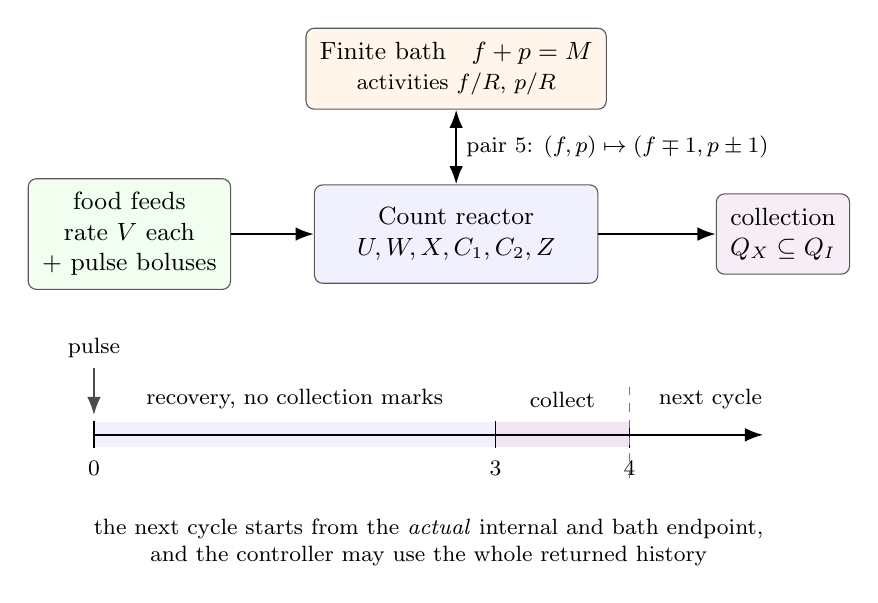
\begin{tikzpicture}[>=Latex,font=\small,
  box/.style={draw=black!65,rounded corners=3pt,align=center,inner sep=5pt},
  bath/.style={box,fill=orange!8},
  rea/.style={box,fill=blue!6,minimum width=3.6cm,minimum height=1.25cm},
  side/.style={box,fill=green!6},
  coll/.style={box,fill=violet!7}]
\node[rea] (R) at (0,0) {Count reactor\\ $U,W,X,C_1,C_2,Z$};
\node[bath] (B) at (0,2.1) {Finite bath\quad $f+p=M$\\ \footnotesize activities $f/R$, $p/R$};
\node[side] (F) at (-4.15,0) {food feeds\\ rate $V$ each\\ + pulse boluses};
\node[coll] (O) at (4.15,0) {collection\\ $Q_X\subseteq Q_I$};
\draw[<->,thick] (R) -- node[right,font=\footnotesize] {pair 5: $(f,p)\mapsto(f\mp1,p\pm1)$} (B);
\draw[->,thick] (F) -- (R);
\draw[->,thick] (R) -- (O);
% ---- protocol timeline, drawn in the same picture at fixed coordinates ----
\begin{scope}[yshift=-2.55cm,font=\footnotesize]
  \fill[blue!6] (-4.6,-0.16) rectangle (0.5,0.16);
  \fill[violet!10] (0.5,-0.16) rectangle (2.2,0.16);
  \draw[->,thick] (-4.6,0) -- (3.9,0);
  \foreach \x/\lab in {-4.6/$0$,0.5/$3$,2.2/$4$} \draw (\x,0.17) -- (\x,-0.17) node[below=1pt] {\lab};
  \draw[->,thick,black!70] (-4.6,0.85) -- (-4.6,0.25);
  \node[anchor=south] at (-4.6,0.85) {pulse};
  \node at (-2.05,0.45) {recovery, no collection marks};
  \node at (1.35,0.45) {collect};
  \node[anchor=west] at (2.45,0.45) {next cycle};
  \draw[dashed,black!55] (2.2,-0.55) -- (2.2,0.7);
\end{scope}
\node[anchor=north,font=\footnotesize,align=center] at (-0.35,-3.5)
  {the next cycle starts from the \emph{actual} internal and bath endpoint,\\
   and the controller may use the whole returned history};
\end{tikzpicture}
\caption{The specified process, not a simulated apparatus. Every driven event moves one molecule between the two bath species; the bath is neither reset nor replenished between cycles, so its composition --- and hence the two directed propensities of pair~5 --- is part of the state carried forward.}
\label{fig:protocol}
\end{figure}

\section{Main results}\label{sec:main}

For cycle $k$ let $S_k$ be the event that its record is successful, $\widehat S_k$ that it is sharply successful, and $E_m=\bigcap_{k\le m}S_k$, $\widehat E_m=\bigcap_{k\le m}\widehat S_k$. Under $\Prob$ a finite sequence of labelled reaction events and pulse outcomes realizing the recorded history exists almost surely; we call it a physical trace. Let $\Pnet$ denote the signed net internal creation of template equivalents along a trace (pair~0 contributes $+1$ forward and $-1$ backward, pair~3 likewise, pair~5 contributes $-1$ forward and $+1$ backward, and pairs~1,2,4 contribute zero). The two error functions $e(V)$ and $\widehat e(V)$ are the explicit finite sums of Appendix~\ref{app:error}.

\begin{theorem}[Finite-bath repeated operation]\label{thm:main}
Fix a bath inventory $M$, parameters satisfying~\eqref{eq:class}, an integer $V\ge V_0:=2\times10^{11}$, an initial full state with $N_0\in\cR_V$, and any controller acting on the returned history. The chronological count process is nonexplosive, and for every $m\in\N$
\begin{equation}\label{eq:probability}
\Prob(E_m)\ \ge\ \bigl(1-e(V)\bigr)^m\ \ge\ 1-m\,e(V),\qquad e(V)\le101\,e^{-V/10^{10}} .
\end{equation}
On $E_m$ all inequalities of~\eqref{eq:success} hold in every cycle, so the mission totals satisfy $\sum_kQ_{I,k}\ge m\lceil V/56\rceil$, $\sum_kQ_{X,k}\ge m\lceil V/1080\rceil$, $\sum_kC_{U,k},\sum_kC_{W,k}\le5mV$ and $\sum_kG_k\le m\lfloor V/5\rfloor$. Displayed linear lower bounds are understood truncated at zero.
\end{theorem}

\begin{theorem}[Sharpened certificate]\label{thm:sharp}
Let $\kappa=\dfrac{1839}{8\,750\,000\,000\,000}=2.1017142857\ldots\times10^{-10}$.
\begin{enumerate}[label=(\alph*)]
\item\label{it:sharp-phase} \emph{(Every admitted bath.)} There is an explicit error sum $\widehat e_\ast(V)\le\widehat e(V)$ for which the conclusion of Theorem~\ref{thm:main} holds verbatim with $e$ replaced by $\widehat e_\ast$, and
\begin{equation}\label{eq:sharpenv}
\widehat e_\ast(V)\ \le\ \widehat e(V)\ \le\ 101\,e^{-\kappa V}\qquad\text{for all }V\ge10^{10}.
\end{equation}
In particular the single-exponential envelope holds from $V\ge10^{10}$, twenty times below the floor $V_0$ needed by~\eqref{eq:probability}, and $\widehat e(V)\le1/100$ for $V\ge5\times10^{10}$.
\item\label{it:sharp-service} \emph{(Pure bath, $d=1/50$.)} If $M=R$ and $d=1/50$, then for every $V\ge10^6$, every admitted incoming full state with $N_0\in\cR_V$ and every intervention, one cycle is \emph{sharply} successful with probability at least $1-\widehat e(V)$; consequently, for $V\ge5\times10^{10}$ and every controller,
\begin{equation}\label{eq:sharpprob}
\Prob(\widehat E_m)\ \ge\ 1-m\,\widehat e(V),
\end{equation}
and on $\widehat E_m$ the mission gross service obeys $\sum_kG_k\le m\lfloor V/10\rfloor$ while all conclusions of Theorem~\ref{thm:main} continue to hold.
\end{enumerate}
\end{theorem}

\begin{theorem}[All-prefix inventory and bath tolerance]\label{thm:prefix}
Let $F_t,P_t$ count the forward and reverse pair-5 events from the start of the mission to a chemical prefix $t$, and $J_t=F_t-P_t$. Then at every supported prefix
\begin{equation}\label{eq:inventory}
f_t=f_0-J_t,\qquad p_t=p_0+J_t,\qquad |J_t|\le F_t+P_t .
\end{equation}
On $E_m$ every prefix, inside cycles as well as at returns, satisfies $|f_t-f_0|=|p_t-p_0|\le B_m:=m\lfloor V/5\rfloor$; on $\widehat E_m$ the same holds with $\widehat B_m:=m\lfloor V/10\rfloor$. Consequently, for a pure bath with $R\ge B_m/\rho$ (respectively $R\ge\widehat B_m/\rho$),
\[
1-\rho\le \frac{f_t}R\le1,\qquad 0\le\frac{p_t}R\le\rho\qquad\text{at every prefix,}
\]
and for the loaded bath both activities lie in $[1-\rho,1+\rho]$, whence for $0<\rho<1$
\[
\Bigl|\log\frac{f_t/R}{p_t/R}\Bigr|\ \le\ \log\frac{1+\rho}{1-\rho}.
\]
\end{theorem}

\begin{corollary}[Explicit inverse design]\label{cor:design}
For $m\ge1$, $0<\delta<1$, $0<\rho<1$ and nonnegative cumulative output demands $D_I,D_X$, put
\begin{equation}\label{eq:design}
V=\max\Bigl\{5\times10^{10},\ \Bigl\lceil\frac{\log(101m/\delta)}{\kappa}\Bigr\rceil,\ \Bigl\lceil\frac{56D_I}m\Bigr\rceil,\ \Bigl\lceil\frac{1080D_X}m\Bigr\rceil\Bigr\},\qquad
R=\max\Bigl\{1,\Bigl\lceil\frac{m\lfloor V/10\rfloor}\rho\Bigr\rceil\Bigr\}.
\end{equation}
Take the pure bath with $r=20$, $d=1/50$ and the all-free-$X$ restart witness. Then with probability at least $1-\delta$, all $m$ cycles are sharply successful, the cumulative collections are at least $D_I$ and $D_X$, and every chemical prefix has fuel activity in $[1-\rho,1]$ and waste activity at most $\rho$.
\end{corollary}
The rule is sufficient and deliberately conservative; it is not a global optimum over reactors or protocols, and the maximum is a design rule, not a necessary condition.

\begin{proposition}[Same-event net synthesis]\label{prop:synthesis}
On $E_m$ a physical trace exists, and every physical trace of the recorded history satisfies
\begin{equation}\label{eq:synthesis}
\Pnet\ \ge\ m\Bigl\lceil\frac V{56}\Bigr\rceil+\Bigl\lceil\frac V{28}\Bigr\rceil-\Iv_{N_0}
\ \ge\ m\Bigl\lceil\frac V{56}\Bigr\rceil+\Bigl\lceil\frac V{28}\Bigr\rceil-\Bigl\lfloor\frac{161V}{160}\Bigr\rfloor
\ \ge\ \Bigl(\frac{m+2}{56}-\frac{161}{160}\Bigr)V .
\end{equation}
In particular $\Pnet>0$ for every $m\ge55$ and every admitted seed, at no probability cost.
\end{proposition}

Proposition~\ref{prop:endpoint} (exact endpoint bath free energies) and Proposition~\ref{prop:metered} (finite metered food) are stated in Section~\ref{sec:consequences}.

\begin{remark}[Quantifiers]\label{rem:quantifiers}
$\Prob$ is the full normalized law; $E_m$ and $\widehat E_m$ are events in it whose probability is bounded below, and nothing is conditioned on success. The parameter class~\eqref{eq:class} is fixed once and is arbitrary within its bounds; in particular $d=0$ is admitted, at which both driven counters vanish identically. The intervention box is available afresh at every cycle and the controller is an arbitrary function of the complete returned history, which now includes the returned bath. The one-cycle bound holds from $V\ge10^6$; the larger floors in~\eqref{eq:probability} and~\eqref{eq:sharpprob} are where the single-exponential envelope and the quantitative corollaries become available.
\end{remark}

\begin{remark}[Two allowances, one law]\label{rem:twoallowances}
Theorem~\ref{thm:sharp}\ref{it:sharp-service} does not weaken Theorem~\ref{thm:main}: $\widehat E_m\subseteq E_m$, and both are events of the same process under the same law. The halved allowance is a \emph{stronger} conclusion bought by a sharper intensity estimate, not a different model or a redefinition of success.
\end{remark}

\section{The one-cycle bound for the changed generator}\label{sec:proof}

This section proves the one-cycle estimate underlying Theorem~\ref{thm:main}. Every statement concerns the full state $(N,f,p)$ and the coefficient rectangle~\eqref{eq:ratebox}; no trajectory of a fixed-activity process is used, and the auxiliary stopped kernels are removed in Section~\ref{sec:transfer} before any conditional repetition.

\subsection{Material control and the retained stock}\label{sec:material}

Internal chemistry preserves both material coordinates, including the driven pair: $X+F\to U+W+P$ moves one $A$-unit and one $B$-unit from $X$ into $U$ and $W$. The only positive material jumps are food arrivals, so direct substitution into~\eqref{eq:generator} gives the exact identities
\begin{equation}\label{eq:drift}
\Lgen A_N=V-A_N,\qquad \Lgen B_N=V-B_N .
\end{equation}
These are unchanged by the bath, which is the first reason the finite-bath problem is tractable.

For the pulse, each material coordinate is a sum of independent retained molecule weights plus an integer food dose. The one-molecule estimate
\[
1-p+p\,e^{-sw}\le\exp\Bigl\{-\Bigl(s-\tfrac{27}{25}s^2\Bigr)pw\Bigr\}\qquad(0\le p\le1,\ 0\le w\le\tfrac95,\ 0\le s\le\tfrac1{10})
\]
applied to the exact product moment generating function of the pulse yields the tails: the admissible bounds put the post-pulse mean of each material coordinate strictly inside $[24V/25,51V/50]$, with weighted exponential bounds giving failure probability at most $4e^{-V/100000}$, while the retained weighted stock has mean at least $\tfrac14\cdot\tfrac{49}{50}\cdot\tfrac V{20}=\tfrac{49V}{4000}$ and lower-tail bound $e^{-1177V/10^9}$ at level $3V/250$ (Appendix~\ref{app:tests}). The exponent uses the actual retained mean rather than a worst-case sum of squared weights.

The analysis is then stopped when either material coordinate leaves $[9V/10,11V/10]$. On this corridor every species count is at most $11V/10$ and the total propensity --- \emph{including} both driven directions, by~\eqref{eq:ratebox} --- is at most $3000V$. This permits uniformization~\citep{jensen1953,grassmann1977}: a Poisson clock of rate $3000V$ selects label $j$ with probability $a_j(s)/(3000V)$ and otherwise makes a null step, with marked counters attached to the selected labels. Exponential tests for the deviations in~\eqref{eq:drift} bound exit during the required time by
\begin{equation}\label{eq:Mterm}
M(V)=4e^{-V/2000}+48000\,V\,e^{-V/2000+1/50},
\end{equation}
and the same mean-reverting drift with a time-dependent tilt returns $A,B$ to their narrow restart bands at time $4$ apart from $4(e^{-V/320000}+e^{-V})$ and the already accounted corridor exits.

\subsection{Recovery and residence of the weighted catalyst}\label{sec:recovery}

The weighted stock $Y$ is chosen so that successive catalytic phases contribute positive drift below a small threshold. Direct source algebra gives the exact identity
\begin{equation}\label{eq:Ydrift}
\Lgen Y_N=V\,Y\bigl(f_{r,\alpha,\beta}(N/V)\bigr)+\frac{rN_X}{5V},
\end{equation}
where $f_{r,\alpha,\beta}$ is the mass-action concentration field of Table~\ref{tab:rates} with the \emph{instantaneous} coefficients $\alpha=df/R$, $\beta=d\eta p/R$ evaluated at the current bath, and the last term is the exact favourable falling-factorial correction. No derivative of a frozen-bath approximation is taken: the generator acts on an internal observable at the full current state, and the bath enters only through $(\alpha,\beta)$, which~\eqref{eq:ratebox} confines to a rectangle. On the material corridor and below the threshold $Y_N\le3V/50$ the parameter bounds give
\begin{equation}\label{eq:Ypositive}
\Lgen Y_N\ \ge\ \tfrac23\,Y_N .
\end{equation}
This is a generator inequality, not a claim that each random path grows monotonically. Weighted jumps have magnitude at most $9/5$ and their rate-weighted squares are bounded by a linear function of $Y_N$ plus the basal source, so exponentially tilted tests convert the positive drift into a lower-tail estimate for entry into $Y\ge3V/50$: a backward tilt schedule with exponential-drift coefficient $5/8$, transported from $1/1000$ at the deadline and capped at $101/20000$, gives failure to enter by time $11/4$, before material exit, at most $e^{-3V/5\cdot10^6}+e^{-V/2}$. A second tilted test controls descent from $3V/50$ to $V/20$ through the remaining $5/4$ time units, contributing $e^{-V/10000}+12000Ve^{-V/10000+9/500}$. Together with~\eqref{eq:Mterm} these form the term $R_{\mathrm{err}}(V)$ of Appendix~\ref{app:error}. The times $11/4$ and $1/4$ partition the analysis only; the physical uncollected run lasts three units.

\subsection{Positive phase transport to free product}\label{sec:phase}

Large weighted stock does not mean large free $X$ at the same instant, and this gap supplies the dominant error term. On the material corridor the coordinate drifts satisfy
\begin{equation}\label{eq:phasedrift}
\begin{aligned}
\Lgen N_X&\ge-70N_X+20N_{C_1}+38N_Z, &\qquad \Lgen N_{C_2}&\ge-70N_{C_2},\\
\Lgen N_{C_1}&\ge-70N_{C_1}+20N_{C_2}, &\qquad \Lgen N_Z&\ge-70N_Z+20N_{C_2},
\end{aligned}
\end{equation}
with all off-diagonal coefficients nonnegative. Put $q_c=3000V$, $a=1-70/q_c$, and initialize a backward weight vector at $(1,0,0,0)$ on $(X,C_1,C_2,Z)$. One clock step maps $w$ to
\[
\bigl(aw_X,\ aw_{C_1}+20w_X/q_c,\ aw_{C_2}+20(w_{C_1}+w_Z)/q_c,\ aw_Z+38w_X/q_c\bigr),
\]
so the weights remain nonnegative with sum at most one, and after $n$ steps equal
\begin{equation}\label{eq:weights}
a^n\Bigl(1,\ \frac{20n}{q_ca},\ \frac{580\,n(n-1)}{q_c^2a^2},\ \frac{38n}{q_ca}\Bigr).
\end{equation}
For $89V\le n\le91V$ elementary bounds on $a^n$ give $w(n)\cdot N\ge Y_N/35$: every catalytic phase funds a future free-$X$ observation, so the estimate does not assume that stock is initially free. Figure~\ref{fig:phase} plots these weights.

To control fluctuations, apply~\eqref{eq:generator} to $e^{-s\,w\cdot N}$. The jump bound and the total rate give the explicit quadratic remainder
\begin{equation}\label{eq:quadratic}
\Lgen e^{-s\,w\cdot N}\le e^{-s\,w\cdot N}\bigl\{-sD_w(N)+7200Vs^2\bigr\},\qquad 0\le s\le\tfrac1{100},
\end{equation}
$D_w$ being the weighted right side of~\eqref{eq:phasedrift}. Iterating with the backward weights at $s=10^{-6}$, the transported lower bound $w(n)\cdot N\ge V/700$ (from $Y\ge V/20$) dominates the low-$X$ threshold $N_X\le V/1000$ and the accumulated quadratic remainder $(12/5)\cdot91V s^2$. The resulting probability of low free $X$ while the path remains active is $e^{-\kappa V}$ with $\kappa$ as in Theorem~\ref{thm:sharp}; Section~\ref{sec:sharp-phase} is devoted to keeping this constant rather than rounding it to $10^{-10}$.

At every later clock time the same bound applies, and summing expectations with Markov's inequality shows that low-$X$ states occupy at most one percent of collection clock steps except with probability $100e^{-\kappa V}$; this step requires no independence between those states. A marked exponential test for actual $X$ washouts then produces the free-output failure bound on the active path.

\subsection{Other marked outputs and expenses}\label{sec:counters}

Template washout has intensity $\Iv_N$, and the coordinatewise comparison $Y_N\le\tfrac75\Iv_N$ obtained from the four coefficients in~\eqref{eq:observables} gives $\Iv_N\ge V/28$ throughout residence above $Y=V/20$. The marked count test yields template-output failure at most $e^{-V/100000}$, including the one-count margin needed to certify the integer ceiling.

Food additions cost at most $151V/200$ per species from the pulse; each feed has constant rate $V$ for four units, and exponential upper-tail tests give $e^{-V/300}$ per food ceiling $5V$. For the gross driven counter, the material corridor gives
\begin{equation}\label{eq:grossnaive}
\alpha N_X+\beta N_UN_W/V\ \le\ \Bigl(\frac1{25}\cdot\frac{11}{10}+\frac1{200\,000\,000\,000}\cdot\frac{121}{100}\Bigr)V\ <\ \frac9{200}V,
\end{equation}
and the marked upper-tail test with a one-count floor gives $e^{-V/2000}$ for the ceiling $\lfloor V/5\rfloor$. Section~\ref{sec:sharp-service} replaces~\eqref{eq:grossnaive} by a strictly better estimate.

All five counters are functions of the same sequence of labelled events, so adding their failure probabilities is a union bound within one joint law, never a product of marginals.

\subsection{Removing the stopping and identifying the physical law}\label{sec:transfer}

The finite stopped process is an analytical device, and transferring its estimates requires care. We use the \emph{strict} event on which the terminal state is still active, in addition to the output and restart conditions. Inactive states are absorbing in the stopped kernel, so terminal activity implies that no earlier exit occurred; on this event the stopped and literal updates --- including bath updates and counter increments --- agree at every step. A small exact model shows this is necessary: for a closed restart event the stopped probability can be $1$ while the physical probability is $1/2$, whereas the strict event gives $1/4$ for both.

For a finite region with bounded rates, both the uniformized marked kernel and the chronological jump construction satisfy the same first-event renewal equation; expanding on the first waiting time and label gives that equation directly, and uniqueness follows by iterating the residual on a bounded time interval, whose remainder is bounded by the corresponding exponential-series tail. Hence the two killed laws agree, preserving waiting times and labels, not merely a state marginal.

To pass to the countable state space, exhaust it by material-height regions. On a bounded interval only the two constant-rate food feeds can increase total material, so their number is almost surely finite; the bath contributes only $M+1$ values. Every material-height region therefore contains finitely many full states and has bounded total rate, so explosion is impossible, and increasing killed endpoint laws exhaust the unrestricted chronological law. Their deterministic-time composition identities pass to the limit by monotone convergence, so the analytical split $11/4+1/4$ is exactly the physical three-unit recovery law followed by the one-unit marked collection.

Integrating over the normalized molecule-pulse distribution --- no bad pulse and no failed source path is removed --- gives the conditional one-cycle bound: for $V\ge10^6$, every restart state, every admitted bath and every intervention,
\begin{equation}\label{eq:onecycle}
\Prob\bigl(S_1\mid N_0,f_0,\text{intervention}\bigr)\ \ge\ 1-e(V).
\end{equation}

\subsection{Conditional histories and the product bound}\label{sec:repeat}

Write $K(h,\cdot)$ for the next-history kernel, built from the actual full endpoint and the policy choice at $h$. A successful return has internal state in $\cR_V$ while its retained bath still satisfies $f+p=M$, so~\eqref{eq:onecycle} applies again at that history. With $S$ the event that the newest cycle succeeds,
\begin{equation}\label{eq:induction}
\Prob(E_{m+1})=\int_{E_m}K(h,S)\,d\Prob(h)\ \ge\ \bigl(1-e(V)\bigr)\Prob(E_m),
\end{equation}
and induction with Bernoulli's inequality proves~\eqref{eq:probability}. This iterates a \emph{conditional} bound; it assumes neither independence of cycles nor renormalization after rejecting failures, and the restricted history measure is a submeasure of the full law throughout. Almost-sure existence of physical traces is preserved under the iteration.

Finally, at each forward event $f$ decreases by one and $p$ increases by one, with signs reversed at each reverse event; induction on the actual labelled trace gives the first two identities of~\eqref{eq:inventory}. Pulses leave the bath unchanged. At every chemical prefix the absolute signed change is bounded by the number of driven events seen so far, which is no larger than the final mission gross count because the marks are nonnegative --- this is what upgrades an endpoint statement to an all-prefix statement. Summing the per-cycle gross bounds proves Theorem~\ref{thm:prefix}; division by $R$ gives the activity corridors, and the loaded-bath force bound follows from $\log$ monotonicity.

\section{Two refinements of the certificate}\label{sec:sharp}

Sections~\ref{sec:sharp-phase} and~\ref{sec:sharp-service} contain the new mathematics of this paper. They are independent: the first reduces the copy scale needed for a given confidence, the second halves the reservoir needed for a given copy scale, and Section~\ref{sec:sharp-compose} composes them.

\subsection{The unrounded phase exponent and a new absorption estimate}\label{sec:sharp-phase}

\begin{lemma}[Exact phase rate]\label{lem:kappa}
At tilt $s$, transported stock lower bound $V/700$, low-$X$ threshold $V/1000$, at most $91V$ clock steps and quadratic remainder $(12/5)s^2$ per step, the exponent of the phase estimate of Section~\ref{sec:phase} is $-\kappa(s)V$ with
\[
\kappa(s)=s\Bigl(\frac1{700}-\frac1{1000}\Bigr)-\frac{12}5\cdot91\,s^2 .
\]
At the tilt $s=10^{-6}$ used in the proof, $\kappa:=\kappa(10^{-6})=\dfrac{1839}{8\,750\,000\,000\,000}$, exactly $\dfrac{1839}{875}=2.1017\ldots$ times the printed rate $10^{-10}$.
\end{lemma}
\begin{proof}
$\kappa(s)=s\cdot\tfrac3{7000}-\tfrac{1092}5s^2$; at $s=10^{-6}$ this is $\tfrac3{7\cdot10^9}-\tfrac{1092}{5\cdot10^{12}}=\tfrac{1839}{8.75\times10^{12}}$.
\end{proof}

\begin{remark}[Retuning the tilt is nearly exhausted]\label{rem:tilt}
With $\Delta=3/7000$ and $C=(12/5)\cdot91$, the unconstrained maximum of $\kappa(s)=\Delta s-Cs^2$ is at $s_\ast=\Delta/(2C)\approx9.8116\times10^{-7}$, where $\kappa(s_\ast)\approx2.102489\times10^{-10}$. This improves $\kappa$ by about $0.037\%$. A numerical search for a better tilt inside this same inequality therefore cannot remove orders of magnitude; the remaining conservatism is in the inequality --- specifically the worst-case increment used in~\eqref{eq:quadratic} in place of a channelwise rate-weighted squared increment --- and would require a new estimate. Both statements in this remark are conventional arithmetic, replayed by the accompanying script; the improvement carried into the theorems is the recovery of $\kappa$ itself, which is compiled. (Right panel of Figure~\ref{fig:phase}.)
\end{remark}

Carrying $\kappa$ instead of $10^{-10}$ through Section~\ref{sec:phase} is mechanical --- the window bound, the burn-in composition, the occupation estimate and the marked washout test are all monotone in this constant --- but it changes the \emph{envelope}, because the single-exponential form of the certificate is obtained by absorbing every other term of the budget into the phase term. That absorption has to be redone, and it is where the domain floor is determined.

\begin{lemma}[Residual absorption]\label{lem:absorb}
Write $\widehat e(V)$ for the refined budget of Appendix~\ref{app:error}. For every $V\ge0$,
\begin{equation}\label{eq:envelope}
\widehat e(V)\ \le\ 100\,e^{-\kappa V}+2\times10^{6}(V+1)\,e^{-V/(4\times10^{7})},
\end{equation}
and for every $V\ge10^{10}$,
\begin{equation}\label{eq:absorb}
2\times10^{6}(V+1)\,e^{-V/(4\times10^{7})}\ \le\ e^{-\kappa V}.
\end{equation}
Consequently $\widehat e(V)\le101e^{-\kappa V}$ for $V\ge10^{10}$.
\end{lemma}
\begin{proof}
For~\eqref{eq:envelope}: every term of $\widehat e$ other than the phase term $100e^{-\kappa V}$ is of the form $e^{-V/D}$ with $D\le4\times10^{7}$, $e^{-cV}$ with $c\ge1/(4\times10^{7})$, or $cVe^{-V/D+a}$ with $D\le4\times10^{7}$ and $a\le1/50$; since $e^{1/50}\le2$, each is bounded by a constant multiple of $e^{-V/(4\times10^7)}$ or of $V e^{-V/(4\times10^7)}$, and summing the coefficients (Appendix~\ref{app:error}) gives~\eqref{eq:envelope}.

For~\eqref{eq:absorb}, set $c=\tfrac1{4\times10^{7}}-\kappa=\tfrac{216911}{8\,750\,000\,000\,000}$, so that $e^{-V/(4\times10^7)}=e^{-\kappa V}e^{-cV}$ and it suffices that $2\times10^{6}(V+1)\le e^{cV}$. For $V\ge10^{10}$ we have $x:=cV\ge247$, hence $247^{9}x\le x^{10}$, and $x^{10}/10!\le e^{x}$ gives
\[
e^{cV}\ \ge\ \frac{247^{9}c}{3\,628\,800}\,V\ >\ 2.33\times10^{7}\,V\ \ge\ 2\times10^{6}(V+1),
\]
the last step because $V\ge10^{10}$. The margin is a factor above $11$, so the floor $10^{10}$ is comfortable rather than tight.
\end{proof}

Two consequences deserve emphasis. First, the floor for the single-exponential form drops from $2\times10^{11}$ to $10^{10}$; the larger floor $5\times10^{10}$ quoted in Theorem~\ref{thm:sharp} is what makes $\widehat e(V)\le1/100$, i.e.\ what makes the linear bound informative, not what makes the envelope valid. Second, the useful confidence threshold moves: $101\,m\,e^{-\kappa V}\le\delta$ now solves to $V\ge\kappa^{-1}\log(101m/\delta)$ with $\kappa^{-1}=4.758\times10^{9}$ instead of $10^{10}$.

\subsection{Correlated bath fractions halve the service allowance}\label{sec:sharp-service}

The estimate~\eqref{eq:grossnaive} bounds each directed coefficient by its own maximum over the admissible class. For the pure bath that is wasteful, because the two coefficients are not free: $f+p=R$ forces $a:=f/R$ and $b:=p/R$ to satisfy $a+b=1$ at every reachable composition.

\begin{lemma}[Correlated gross envelope]\label{lem:envelope}
Let $M=R$, $d=1/50$. On the material corridor $N_U,N_W,N_X\le\tfrac{11}{10}V$, the total gross driven intensity satisfies
\begin{equation}\label{eq:grosssharp}
\alpha N_X+\beta\frac{N_UN_W}V\ =\ \frac1{50}\Bigl(a\,N_X+\eta\,b\,\frac{N_UN_W}{V}\Bigr)\ \le\ \frac{11}{500}\,V .
\end{equation}
\end{lemma}
\begin{proof}
With $u=N_U/V$, $w=N_W/V$, $x=N_X/V$ all at most $11/10$, we have $\eta uw\le\eta(11/10)^2\le11/10$, so $ax+\eta b\,uw\le(a+b)\cdot\tfrac{11}{10}=\tfrac{11}{10}$, and the factor $1/50$ gives~\eqref{eq:grosssharp}. The point is that $a$ and $b$ are weights of a convex combination, whereas~\eqref{eq:grossnaive} maximizes them separately.
\end{proof}
The gain over~\eqref{eq:grossnaive} is the factor $\tfrac{11}{500}\big/\tfrac9{200}=\tfrac{44}{90}$, slightly better than a half.

\begin{lemma}[Sharp service tail]\label{lem:sharptail}
Under the hypotheses of Lemma~\ref{lem:envelope}, for the three-stage stopped marked source over the four time units and every incoming full state,
\[
\Prob\Bigl(G\ \ge\ \frac V{10}-1\Bigr)\ \le\ \exp\Bigl\{-\frac1{10}\Bigl(\frac V{10}-1\Bigr)+4\cdot\frac{11}{500}V\bigl(e^{1/10}-1\bigr)\Bigr\}\ \le\ e^{-V/2000}\qquad(V\ge10^6).
\]
\end{lemma}
\begin{proof}
Uniformization turns the intensity bound~\eqref{eq:grosssharp} into a one-step multiplicative bound for the mark-generating function; composing the three stages and applying the exponential Markov inequality at tilt $s=1/10$ gives the displayed exponent. Using $e^{1/10}-1\le\tfrac{53}{500}$,
\[
-\frac V{100}+\frac{11V}{125}\cdot\frac{53}{500}=-\frac{21V}{31250},
\]
and $\tfrac{21}{31250}>\tfrac1{2000}$ absorbs the one-count rounding buffer for $V\ge10^6$.
\end{proof}

\begin{remark}[A first attempt that fails, and why it matters]\label{rem:failed}
Reusing the independent cap $\tfrac9{200}V$ with the same tilt gives exponent $-\tfrac V{100}+4\cdot\tfrac9{200}V\cdot\tfrac{53}{500}=+\tfrac{227V}{25000}>0$: no tail at all. The correlated envelope is therefore not a cosmetic improvement of constants but the step that makes the halved allowance provable, and the failure of the independent version is a weak estimate, not a counterexample.
\end{remark}

\paragraph{From a tail to an exported conclusion.}
Lemma~\ref{lem:sharptail} alone does not prove Theorem~\ref{thm:sharp}\ref{it:sharp-service}. The success predicate $\lfloor V/5\rfloor$ is fixed inside the prepared-cycle failure union, the strict stopped-to-physical transfer, the literal-cycle bound, the returned-history iteration and the prefix sizing corollary; supplying a stronger local inequality to a theorem whose stated conclusion still reads $\lfloor V/5\rfloor$ proves nothing. Accordingly we rebuild that chain around the smaller event. Define the sharp failure set as the original prepared-cycle failure union together with $\{G\ge V/10-1\}$, so that its complement gives cycle success \emph{and} $G\le\lfloor V/10\rfloor$; bound its pulse-integrated probability by $\widehat e_\ast(V)+e^{-V/2000}$ using the union bound on the one joint law, transfer it through the strict active event to the literal chronological cycle exactly as in Section~\ref{sec:transfer}, and iterate it over returned histories exactly as in Section~\ref{sec:repeat}. Summing the per-cycle sharp gross bounds over the mission and composing with the prefix identity~\eqref{eq:inventory} yields $|f_t-f_0|\le m\lfloor V/10\rfloor$ at every chemical prefix, which is the statement that halves $R$ in Corollary~\ref{cor:design}. Every step of this rebuild is compiled (Appendix~\ref{app:formal}).

\begin{remark}[Scope of the halving]\label{rem:halvescope}
Lemma~\ref{lem:envelope} uses $M=R$ and $d=1/50$. It does not apply verbatim to the loaded bath $M=2R$, where $a+b=2$, nor to $d=1/25$, where the prefactor doubles; for those the allowance $\lfloor V/5\rfloor$ of Theorem~\ref{thm:main} remains the certified value. The phase refinement of Section~\ref{sec:sharp-phase}, by contrast, applies to every admitted bath.
\end{remark}

\subsection{Composing the two refinements}\label{sec:sharp-compose}

The refinements act on different terms of the budget and compose without interaction: the phase refinement changes the constant in the dominant term, the service refinement adds one more exponential of the same magnitude as an already-present term and tightens one conclusion. Writing $\widehat e(V)=\widehat e_\ast(V)+e^{-V/2000}$ for the combined budget, Lemma~\ref{lem:absorb} covers both, and Theorem~\ref{thm:sharp} follows by the composition of Sections~\ref{sec:transfer} and~\ref{sec:repeat}. The resulting design rule is Corollary~\ref{cor:design}; Figure~\ref{fig:certificate} compares the two certificates and the two reservoir rules.

\begin{figure}[tb]
\centering

\includegraphics[width=\linewidth]{certificate.pdf}
\caption{Left: the hundred-cycle failure bound $101\,m\,e^{-\kappa V}$ against the rounded $101\,m\,e^{-V/10^{10}}$; the dotted line is the confidence of the original certified instance, which the refined bound reaches at $V=9.6\times10^{10}$. Right: sufficient pure fuel $R$ against mission length at $\delta=10^{-2}$, $\rho=10^{-1}$ and no additional output demand, under the two per-cycle allowances; markers are the two certified hundred-cycle instances. Both panels evaluate proved bounds; integer rounding is retained in the certified instances but not in the plotted curves.}
\label{fig:certificate}
\end{figure}

\begin{figure}[tb]
\centering

\includegraphics[width=\linewidth]{phase.pdf}
\caption{Left: the backward phase-transport weights~\eqref{eq:weights} in their large-$V$ form, with the observation window shaded and the certified coefficient $1/35$ marked; $w_{C_2}$ is scaled by $10^3$ to be visible. Right: the phase exponent $\kappa(s)$ of Lemma~\ref{lem:kappa}; the tilt actually used already attains $2.1017\times10^{-10}$, and the optimum of this parabola improves it by under $0.04\%$.}
\label{fig:phase}
\end{figure}

\section{Inventory, design and thermochemical consequences}\label{sec:consequences}

\subsection{Terminal stock strengthens net synthesis}\label{sec:netsynth}

\begin{proof}[Proof of Proposition~\ref{prop:synthesis}]
Telescoping the template inventory along the literal reactions and pulse outcomes gives, for every physical trace,
\[
\Pnet=\Iv_{\mathrm{final}}-\Iv_{N_0}+Q_{\text{all washout}}+\Iv_{\text{withdrawn}}+\Iv_{\text{extra loss}} .
\]
All removed inventories are nonnegative and food boluses contain no templates, so the collected output during the designated windows --- a subset of all washout --- may be substituted as a lower bound. Comparing the four coefficients in~\eqref{eq:observables} gives $40Y_N\le56\Iv_N$, so the restart condition $Y\ge V/20$ forces $\Iv_{\mathrm{final}}\ge\lceil V/28\rceil$. Initially $\Iv_{N_0}\le A_{N_0}\le\lfloor161V/160\rfloor$ with integer inventory. These give the first two bounds; relaxing the ceilings and the floor gives the third, whose coefficient at $m=55$ is $13/1120>0$ while at $m=54$ it is negative.
\end{proof}
The statement is that the entire certified output cannot be accounted for by harvesting the initial seed. It does not identify the ancestry of individual molecules, and it is not a statement about net fuel consumption: the two are different observables, related only through the driven pair.

\subsection{Exact finite-bath thermochemistry}\label{sec:thermo}

Use dimensionless free energies in units of $k_BT$. For a species of count $n$, standard potential $g$ and reference count $C>0$ set
\begin{equation}\label{eq:potential}
\phi(n;g,C)=ng+\log(n!)-n\log C .
\end{equation}
The internal standard potentials are those of the chemical realization~\citep{thermo2026},
\[
(g_U,g_W,g_X,g_{C_1},g_{C_2},g_Z)=(0,\,0,\,-\log10,\,-\log10,\,-\log10,\,-2\log10),
\]
and the bath potentials are $g_F=A_0:=\log(8\times10^{10})$ and $g_P=0$, with equal reference counts $R$.

\begin{proposition}[Neighbouring-state local detailed balance]\label{prop:ldb}
For a supported forward driven step from $(u,w,x,f,p)$ with $x,f\ge1$ and $d>0$, evaluating the reverse propensity at the post-forward state $(u+1,w+1,x-1,f-1,p+1)$ gives
\begin{equation}\label{eq:ldb}
\frac{a_+(s)}{a_-(s+\nu_+)}=8\times10^{9}\cdot\frac{f}{p+1}\cdot\frac{R_P}{R_F}\cdot\frac{Vx}{(u+1)(w+1)}=\exp\{-\Delta G_{\mathrm{total}}\},
\end{equation}
with $\Delta G_{\mathrm{total}}$ computed from~\eqref{eq:potential} over the five changing species.
\end{proposition}
The identity $\phi(n+1)-\phi(n)=g+\log(n+1)-\log C$ applied to each changing species gives~\eqref{eq:ldb} directly. The neighbouring convention matters: at $p=0$ the post-state has $p+1=1$, so no chemical potential is evaluated at $\log 0$, whereas a same-state forward/reverse ratio is undefined there. At $d=0$ the pair is inactive and no ratio of vanishing propensities is asserted.

\begin{proposition}[Endpoint bath free energies]\label{prop:endpoint}
Let $J=F-P$ be the net forward driven service over a mission and $W_b$ the bath free-energy decrease. From a pure bath $(R,0)$ one has $0\le J\le R$ and
\begin{equation}\label{eq:pureenergy}
\Delta G_b=-A_0J-\log\binom RJ,\qquad \frac{W_b}{k_BT}=A_0J+\log\binom RJ .
\end{equation}
From a loaded bath $(R,R)$ one has $-R\le J\le R$ and
\begin{equation}\label{eq:loadedenergy}
\Delta G_b=-A_0J+\log\frac{(R-J)!\,(R+J)!}{(R!)^2}.
\end{equation}
\end{proposition}
\begin{proof}[Proof (conventional algebra from the compiled potential and inventory identities)]
The exact inventory identity~\eqref{eq:inventory} gives final bath counts $(R-J,J)$ in the pure case. Subtracting $\phi(R;A_0,R)+\phi(0;0,R)$ from the endpoint potential leaves $-A_0J+\log((R-J)!)+\log(J!)-\log(R!)$, the reference-count terms cancelling because the total bath inventory is conserved; the factorial definition of $\binom RJ$ gives~\eqref{eq:pureenergy}. The loaded endpoint is $(R-J,R+J)$ and the same cancellation gives~\eqref{eq:loadedenergy}. All factorial arguments are nonnegative integers, including at the boundaries, and $0!=1$.
\end{proof}
No fixed affinity and no Stirling approximation is used. Three distinctions must stay explicit: gross turnover $F+P$ is not net conversion $J$; a bath free-energy decrease is not extracted useful work; and detailed balance for the reversible chemistry does not account for pumping, feeding, withdrawal, separation, timing or thermal control. The bath is closed to replenishment, but the reactor-plus-apparatus system is not a closed autonomous chemical system~\citep{rao2018,esposito2012}.

\begin{corollary}[Force-budget inversion]\label{cor:force}
For the loaded bath put $b=\widehat B_m/R$. Requiring the dimensionless affinity drift to be at most $\zeta>0$ is certified by $2\operatorname{artanh}(b)\le\zeta$, i.e.\ by
\[
R\ \ge\ \widehat B_m\coth(\zeta/2),
\]
with integer rounding applied afterwards. At $\zeta=0.1$ this is $R/\widehat B_m\ge20.0167$; at $\zeta=0.02$, $R/\widehat B_m\ge100.0034$.
\end{corollary}
This gives a thermodynamic design knob in place of an arbitrary percentage tolerance. It does not apply to ``deviation from the initial pure-bath affinity'', since that macroscopic log ratio is singular at zero initial waste. For general initial loadings $f_0,p_0>0$ with $|J|\le B<\min(f_0,p_0)$ the affinity change is exactly $\Delta A(J)=\log(1-J/f_0)-\log(1+J/p_0)$, decreasing in $J$, so its worst absolute value over $[-B,B]$ is $\max\{\log\frac{1+B/p_0}{1-B/f_0},\log\frac{1+B/f_0}{1-B/p_0}\}$; if a one-sided preparation constrains $J$, intersect with its support before taking extrema rather than charging impossible directions. (Conventional deterministic consequences of~\eqref{eq:inventory}.)

\subsection{Finite metered food}\label{sec:metered}

\begin{proposition}[Metered no-stockout]\label{prop:metered}
Let $P_U,P_W$ be the food separately charged to the chosen preparation, and allocate initial stocks $H_U=P_U+5mV+1$ and $H_W=P_W+5mV+1$. Let an external metering mechanism supply each original arrival clock at intensity $V$ while stock remains, pay the literal pulse boluses, and move to an absorbing shutdown if a requested delivery cannot be funded. Then the metered mission succeeds with at least the probability given by Theorem~\ref{thm:main} (respectively Theorem~\ref{thm:sharp}), and all finite-bath prefix and activity consequences hold on the same event.
\end{proposition}
\begin{proof}[Proof (compiled inventory and rate agreement; conventional path coupling)]
That the full propensity vector of the metered process agrees with the original before stockout, and that the cumulative counters are nondecreasing at chemical, cycle and mission prefixes with the boluses included, are compiled. For the transfer, construct both processes with common randomness: while their full states agree and both stocks are positive, use the same exponential waiting draw and the same label draw --- their propensity vectors agree there, so time, label, internal update and bath update agree --- and the same pulse outcome at each intervention, debiting the specified integer boluses. Nonexplosion (Section~\ref{sec:transfer}) makes this recursion well defined through the finitely many jumps and the finitely many pulses of a bounded mission. On the original success event, cumulative use of each food is at most $5mV$ at every prefix, so the spare molecule keeps both stocks strictly positive and no shortage occurs; the coupled processes then agree in all states, labels, times and collected outputs, and the original success event is contained in the metered one.
\end{proof}
A passive food tank whose arrival intensity declines with its remaining concentration is a different model and is not covered. Finite metered food bounds a prescribed finite mission; it does not make the reactor indefinitely autonomous.

\section{Worked missions, dimensions and diagnostics}\label{sec:examples}

\subsection{Two certified hundred-cycle instances}\label{sec:instances}

Take $m=100$, $\rho=1/10$, $r=20$, $d=1/50$, the pure bath and the all-free-$X$ seed $(0,0,V,0,0,0)$.

\begin{table}[tb]
\centering\footnotesize
\setlength{\tabcolsep}{4.5pt}
\begin{tabular}{lrrr}
\toprule
Quantity & Original certificate & Refined, reduced scale & Refined, original scale\\
\midrule
Copy scale $V$ & $200{,}000{,}000{,}000$ & $96{,}000{,}000{,}000$ & $200{,}000{,}000{,}000$\\
Per-cycle gross allowance & $\lfloor V/5\rfloor$ & $\lfloor V/10\rfloor$ & $\lfloor V/10\rfloor$\\
Pure fuel $R$ at $\rho=1/10$ & $40{,}000{,}000{,}000{,}000$ & $9{,}600{,}000{,}000{,}000$ & $20{,}000{,}000{,}000{,}000$\\
Mission confidence at least & $0.999979$ & $0.999979$ & $1-10^{-13}$\\
Template equivalents collected & $357{,}142{,}857{,}200$ & $171{,}428{,}571{,}500$ & $357{,}142{,}857{,}200$\\
Free $X$ collected (included above) & $18{,}518{,}518{,}600$ & $8{,}888{,}888{,}900$ & $18{,}518{,}518{,}600$\\
Each food, operation only & $\le10^{14}$ & $\le4.8\times10^{13}$ & $\le10^{14}$\\
Gross driven events & $\le4\times10^{12}$ & $\le9.6\times10^{11}$ & $\le2\times10^{12}$\\
Net synthesis, all-free seed & $164{,}285{,}714{,}343$ & $78{,}857{,}142{,}929$ & $164{,}285{,}714{,}343$\\
\bottomrule
\end{tabular}
\caption{One event of the stated probability in each column. The middle column matches the original confidence with $12/25$ of the molecules and $6/25$ of the fuel; the right column keeps the original copy scale and outputs, halves the fuel, and converts the phase refinement into eight further orders of confidence. Output guarantees scale with $V$, so the middle column is not uniformly stronger --- see Remark~\ref{rem:fair}.}
\label{tab:instances}
\end{table}

\begin{remark}[The fair comparison]\label{rem:fair}
Reducing $V$ reduces the certified output at fixed $m$. A user who declares the original output demand $D_I=357{,}142{,}857{,}200$ has $\lceil56D_I/m\rceil>2\times10^{11}$, so the demand term in~\eqref{eq:design} pins the copy scale back at the original value and the improvement is banked entirely as confidence and as reservoir --- the right-hand column of Table~\ref{tab:instances}. The middle column is the correct comparison only when confidence and mission length, not output, are the binding requirements. Holding all of $m$, $\delta$, $D_I$, $D_X$ and $\rho$ fixed, the guaranteed gain of this paper is: the reservoir halves, and the confidence margin improves by the factor $e^{(\kappa-10^{-10})V}$ at whatever $V$ the demands force.
\end{remark}

At every chemical prefix of the middle column, $0.9\le f/R\le1$ and $0\le p/R\le0.1$. The analogous loaded bath has total inventory $2R$, initial fuel and waste $R$ each, the same $d=1/50$, and both activities in $[0.9,1.1]$; by Remark~\ref{rem:halvescope} it keeps the allowance $\lfloor V/5\rfloor$, but it does inherit the phase refinement, so the loaded hundred-cycle mission is certified at $V=9.6\times10^{10}$ with the same confidence $0.999979$ (Appendix~\ref{app:formal}). None of these bath sizes is asserted to be necessary.

\subsection{Which resource controls a mission}\label{sec:resource}

For fixed $V\ge5\times10^{10}$, positive integer $R$, confidence $1-\delta$, tolerance $\rho$ and finite food stocks $H_U,H_W$ with preparation charges $P_U,P_W$, the certified horizon is the minimum of
\begin{equation}\label{eq:budget}
\begin{aligned}
m&\le\Bigl\lfloor\frac\delta{101}e^{\kappa V}\Bigr\rfloor, &\qquad
m&\le\Bigl\lfloor\frac{H_U-P_U-1}{5V}\Bigr\rfloor,\\
m&\le\Bigl\lfloor\frac{\rho R}{\lfloor V/10\rfloor}\Bigr\rfloor, &\qquad
m&\le\Bigl\lfloor\frac{H_W-P_W-1}{5V}\Bigr\rfloor .
\end{aligned}
\end{equation}
If $H_i<P_i+1$ the strict no-stockout certificate admits no positive mission; that is infeasibility, not a negative cycle count. Asymptotically, at fixed output demands, $\rho$ and $\delta$, \eqref{eq:design} gives $V=O(1+\log(m/\delta))$ and $R=O\bigl(m(1+\log(m/\delta))/\rho\bigr)$, with food allocations of order $mV$. These are sufficient scaling laws; they establish no matching lower bound and do not rule out a better dependence on $m$ obtained by bounding the largest prefix of the \emph{signed} current $J$ directly through its drift and compensated martingale, instead of through $|J|\le F+P$. For the pure-bath regime, where the reverse coefficient is at most $10^{-11}$ times the forward one, such cancellation is unlikely to help much; that should be diagnosed before a further theorem is attempted.

\subsection{Dimensional reading}\label{sec:units}

Choose reference concentrations $c_\ast$ for the reactor and $c_{b,\ast}$ for the bath, and a kinetic time $\tau$. Then $V=N_Ac_\ast\Omega$, $R=N_Ac_{b,\ast}\Omega_b$ and the mission duration is $4m\tau$; $R$ is not a volume until $c_{b,\ast}$ is specified. At $c_\ast=c_{b,\ast}=1$\,mM and $\tau=60$\,s, the middle column of Table~\ref{tab:instances} has reactor volume $0.159412$\,nL, bath volume $15.9412$\,nL --- a bath-to-reactor ratio of $100$, against $200$ for the original instance --- and a source-running time of $400$ minutes. The corresponding amounts are $0.284664$\,pmol of collected template equivalents, $0.0147604$\,pmol of collected free $X$, at most $79.7059$\,pmol of each food during operation, at most $1.59412$\,pmol of gross driven events (an accounting unit, not a species), and $15.9412$\,pmol of initial pure fuel.

For an order-$k$ internal mass-action term, a dimensionless coefficient $a$ corresponds to $a/(\tau c_\ast^{k-1})$: at these references, a bimolecular $20$ becomes $1000/3\approx333.33\,\mathrm{M^{-1}s^{-1}}$, a unimolecular $20$ becomes $1/3\,\mathrm{s^{-1}}$, and washout becomes $1/60\,\mathrm{s^{-1}}$. The driven pair involves contact between two reference volumes and needs its own explicit convention; the same-volume formula must not be applied mechanically to a separated reservoir. Lowering the concentration at fixed counts is not a free improvement --- it demands different physical rate constants if the dimensionless source is to be unchanged --- and converting counts to nanolitres does not establish a chemical implementation. Mixing, transport across the contact, molecular identities, attainable rate constants, enzyme loadings, osmotic effects and separation efficiency all remain uncalibrated here.

\subsection{Deterministic diagnostics}\label{sec:diagnostics}

\begin{figure}[tb]
\centering

\includegraphics[width=\linewidth]{diagnostics.pdf}
\caption{Deterministic mass-action diagnostics for the reaction table, over eight cycles with retained bath, at $r=20$, $q=1/4$, $\ell_i=49/50$, $e_U=e_W=-1/200$. Left: fuel activity. Right: per-cycle integrated collected template equivalents. The nearly depleted bath ends at fuel activity $2.37\times10^{-10}$ and still collects more per cycle than the abundant cases; the zero-drive case produces output with no driven service at all. These are integrated ODE fluxes, not random counts: they are evidence about mechanism, not about probabilities, attractors or the finite-count theorem.}
\label{fig:diagnostics}
\end{figure}

\begin{center}\small
\begin{tabular}{lrrrrrr}
\toprule
Case & $R/V$ & $d$ & $\min Q_I/V$ & $\min Q_X/V$ & $F/V$ & $P/V$\\
\midrule
Pure & 1 & 0.02 & 0.275215 & 0.128704 & 0.07239 & 1.24e-12 \\
Loaded & 1 & 0.02 & 0.275215 & 0.128704 & 0.07239 & 4.16e-11 \\
Nearly depleted & 0.001 & 0.02 & 0.277266 & 0.129788 & 0.001 & 3.6e-11 \\
Zero drive & 1 & 0 & 0.278579 & 0.130464 & 0 & 0 \\
\bottomrule
\end{tabular}

\captionof{table}{The four diagnostic runs of Figure~\ref{fig:diagnostics}. $F$ and $P$ are mission-integrated directed fluxes. Sampled extrema are diagnostics, not rigorous path bounds.}
\label{tab:diagnostics}
\end{center}

These runs were performed to test one interpretation, namely that sustained output requires abundant fuel, and they reject it for this source: a bath depleted by seven orders of magnitude, and even a bath with the drive switched off entirely, still supports collection at essentially the same level. That is consistent with the structure of the model --- forward drive \emph{destroys} a template --- and it is the reason the theorem's gross allowance is an allowance rather than a requirement.

\section{Scope, limitations and open questions}\label{sec:discussion}

The theorem answers whether a specified reactor can repeatedly recover and deliver output while its finite bath stays inside a requested activity corridor, and how large the preparation, food and bath must be for a declared mission. It does not establish strictly positive net consumption of the named fuel. In this source, forward drive destroys a template and reverse drive creates one; the admitted class includes $d=0$; and a collected-output lower bound is not a lower bound on the preceding occupation integral. A positive net-service theorem would need a quantitative lower bound on integrated free-$X$ occupancy while fuel is sufficiently abundant, a forward-count lower tail, a reverse-count upper tail, and their joint conditional composition. None of these is assumed here, and the compiled conditional obstruction is simply that a premise $J\ge mj_\ast V$ together with $f_{\mathrm{end}}\ge0$ forces $mj_\ast V\le f_0$.

Other explicit non-claims: the effective trimolecular reverse channel has no elementary implementation here; the intervention is instantaneous with conditionally independent thinning; the copy scale is restored externally; and the four-unit clocking is external, so this is not an autonomous system. The model's extreme ratios $\eps$ and $\eta$, the species-dependent loss model and the product-mixture interpretation are at least as consequential for applicability as the copy scale, and a smaller count bound does not address them.

Three directions look worthwhile. (i) The phase estimate still charges every channel a worst-case squared increment; computing the actual rate-weighted quantity $Q_w(N)=\sum_ja_j(N)(w\cdot\nu_j)^2$ channel by channel --- food feeds and food washout contribute zero to an internal catalytic observable, $Z\rightleftharpoons2X$ contributes $(2w_X-w_Z)^2$, the driven pair contributes $w_X^2$ times its gross intensity --- and integrating a certified envelope along the adjoint schedule would sharpen~\eqref{eq:quadratic} where Remark~\ref{rem:tilt} shows retuning cannot. (ii) Targeting the integrated free-$X$ occupation or the collection count directly with a backward equation carrying a reward term may avoid paying for pointwise low-$X$ events and then applying Markov's inequality; an earlier constant-corrector attempt failed on endpoint penalties, so time-dependent weights and all boundary terms must be retained. (iii) A signed-current estimate for $\sup_t|J_t|$, as discussed in Section~\ref{sec:resource}, would improve the reservoir rule if directional cancellation is significant. After any such improvement the whole budget must be recomputed: once the phase term is reduced, $e^{-V/(4\times10^{7})}$ becomes the next obstruction, and a small exponent improvement must never be advertised as a many-orders-of-magnitude copy-number result.

Finally, formal verification supports the theorems under their stated hypotheses. It says nothing about whether those hypotheses describe a particular piece of chemistry, and the calibration questions listed in Section~\ref{sec:units} are precisely the ones that must be settled before this certificate is applied to a real biochemical process.

\appendix

\section{Complete error budgets}\label{app:error}

For $V\ge0$ define
\begin{align*}
M(V)&=4e^{-V/2000}+48000\,V\,e^{-V/2000+1/50},\\
R_{\mathrm{err}}(V)&=e^{-3V/5000000}+e^{-V/2}+M(V)+e^{-V/10000}+12000\,V\,e^{-V/10000+9/500},\\
F(V)&=e^{-V/40000000}+100\,e^{-V/10^{10}}+e^{-V}+e^{-V/200},\\
J_{\mathrm{err}}(V)&=F(V)+e^{-V/100000}+2e^{-V/300}+e^{-V/2000},\\
T(V)&=M(V)+R_{\mathrm{err}}(V)+4\bigl(e^{-V/320000}+e^{-V}\bigr),\\
e(V)&=e^{-1177V/10^{9}}+4e^{-V/100000}+J_{\mathrm{err}}(V)+T(V).
\end{align*}
Here $M,R_{\mathrm{err}},F,J_{\mathrm{err}},T$ are error functions, not the bath inventory, capacity, directed counters or net service; $J_{\mathrm{err}}$ is the joint five-counter budget and $T$ the restart budget, and the pulse terms sit outside the prepared-cycle budget. This is exactly the one-cycle error of Theorem~\ref{thm:main}, with repeated material terms retained rather than silently optimized away.

The refined budget replaces the single phase term and adds the sharp service term:
\[
\widehat F(V)=e^{-V/40000000}+100\,e^{-\kappa V}+e^{-V}+e^{-V/200},
\]
with $\widehat J_{\mathrm{err}},\widehat e_\ast$ defined from $\widehat F$ exactly as $J_{\mathrm{err}},e$ are defined from $F$, and $\widehat e(V)=\widehat e_\ast(V)+e^{-V/2000}$. Every exponential besides the phase term is bounded by a multiple of $e^{-V/(4\times10^{7})}$, and the two positive offsets have exponent at most $1/50$ with $e^{1/50}\le2$; summing coefficients gives~\eqref{eq:envelope}, and~\eqref{eq:absorb} completes Lemma~\ref{lem:absorb}. For the original budget the analogous statement is $e(V)\le100e^{-V/10^{10}}+10^{6}(V+1)e^{-V/(4\times10^{7})}$ with absorption valid from $V\ge2\times10^{11}$, which is the origin of the floor $V_0$.

Numerically, at $V_0=2\times10^{11}$ one has $e^{20}\ge\sum_{k=0}^{36}20^k/k!>4.848\times10^{8}$, so $e(V_0)\le101/(4.848\times10^{8})$ and $100\,e(V_0)\le21/10^{6}$. For the refined budget at $V=9.6\times10^{10}$ we have $\kappa V\ge20$, giving the same $21/10^{6}$; and at $V=2\times10^{11}$ we have $\kappa V\ge42$ and $e^{42}\ge(e^{20})^2\ge2.3503\times10^{17}$, giving $100\,\widehat e(V)\le10^{-13}$. At $V=5\times10^{10}$, $\kappa V\ge10$ and $e^{10}\ge10100$ give $\widehat e(V)\le1/100$. These are rational comparisons against positive Taylor sums, not rounded numerical exponentials.

\section{Quantitative exponential tests}\label{app:tests}

For a stopped bounded-rate source and a linear observable $H$, the exponential test obeys
\begin{equation}\label{eq:testidentity}
\frac{\Lgen e^{sH(N)}}{e^{sH(N)}}=\sum_ja_j(N)\bigl(e^{s\Delta_jH}-1\bigr).
\end{equation}
On the small arguments used here, $e^z\le1+z+\tfrac35z^2$ for $|z|\le\tfrac9{50}$, so drift plus the rate-weighted sum of squared jumps bounds~\eqref{eq:testidentity}. Uniformization turns a generator bound into a one-step multiplicative bound; iteration, the exponential Markov inequality and Poisson summation supply the stated tails, and indicators of activity kill a test on exit, every resulting exit probability being included explicitly in $M,R_{\mathrm{err}},T$.

\paragraph{Pulse.}
For independent Bernoulli retention indicators $B_a$ and nonnegative weights $w_a$, $\E\exp(s\sum_aw_aB_a)=\prod_a(1-p_a+p_ae^{sw_a})$. With material weights at most $2$ and stock weights at most $9/5$, the parameter bounds give unrounded pulse material means in $[31213V/32000,3231V/3200]$, and a food floor lowers a mean by less than one, leaving for $V\ge10^6$ the slack required for $[24V/25,51V/50]$. For stock, $1-p+pe^{-sw}\le\exp\{-(s-\tfrac{27}{25}s^2)pw\}$ for $0\le w\le9/5$, $0\le s\le1/10$; at $s=1/100$ with $\sum_ap_aw_a\ge49V/4000$ and level $3V/250$ the exponent is exactly $-1177V/10^{9}$. Either bad material band requires a centred deviation of magnitude at least $V/100$, giving $e^{-V/100000}$ per sign and coordinate.

\paragraph{Material corridor and terminal return.}
For each material coordinate use the barriers $U_H=e^{(H-11V/10)/100}$ and $L_H=e^{-(H-9V/10)/100}$. Their sum is at least one on exit and at most $4e^{-V/2000}$ at a prepared start; on the stopped corridor each barrier has generator at most $3000Ve^{-V/2000+1/50}$, and integration for time $4$ gives $M(V)$. For terminal return, the compensated tilt contracts the test parameter by $1-1/(3000V)$ per clock step, so for $n\ge11700V$ the contraction factor is at most $1/40$; taking $s=\pm1/1000$ with $|H_0-V|\le V/25$ gives exponent at most $-V/320000$ for the threshold $|H-V|\ge V/160$, and the clock of mean $12000V$ misses its cutoff with probability at most $e^{-V}$.

\paragraph{Recovery and residence.}
Below $3V/50$ the drift~\eqref{eq:Ypositive} plus its bounded-jump quadratic remainder gives $\Lgen e^{-sY}\le-\tfrac58sYe^{-sY}$ for $0\le s\le1/100$; the tilt transported backward over $8100V$ steps from $1/1000$ reaches its cap because $(1+\tfrac{5/8}{3000V})^{8100V}\ge(17/16)^{27}>101/20$, and the exponential Markov inequality at prepared stock $3V/250$ gives $e^{-3V/5\cdot10^6}$, while a Poisson clock of mean $8250V$ falls below $8100V$ with probability at most $e^{-V/2}$. For continued residence, $H_Y=\max(e^{-Y/100},e^{-3V/5000})$ has generator at most $3000Ve^{-3V/5000+9/500}$, giving the lower-exit bound $e^{-V/10000}+12000Ve^{-V/10000+9/500}$.

\paragraph{Phase margin and collection.}
In~\eqref{eq:weights}, $a^n\ge1/12$ for $n\le91V$, and $n\ge89V$, $n-1\ge88V$ give each coefficient at least $1/35$ times its stock weight. The phase exponential remainder per clock step is $(12/5)s^2$, so at $s=10^{-6}$ its total over $91V$ steps is $(12/5)\cdot91V\cdot10^{-12}$; with the low-$X$ threshold contributing $V/10^{9}$ and the initial stock $-V/(700\cdot10^{6})$, the combined exponent is at most $-\kappa V$, which is the content of Lemma~\ref{lem:kappa}. After a burn-in of at least $90V$ clock steps this bounds low-free occupancy at every later step; if $B$ counts bad steps among $n$ collection steps then $\E B\le ne^{-\kappa V}$ and $\Prob(B\ge n/100)\le100e^{-\kappa V}$. A marked tilt of size $1/1000$ for free washouts then gives the joint shortfall bound
\[
\exp\Bigl\{\frac1{1000}\Bigl(K+\frac{B_\ast}{3000000}\Bigr)-\frac{33n}{10^{11}}\Bigr\}+\Prob(B\ge B_\ast),
\]
with $K=V/1080+1$, $B_\ast=n/100$ and $n\ge2990V$; for $V\ge10^6$ the first term is at most $e^{-V/(4\times10^7)}$, and the precollection quarter-unit and collection unit clocks of means $750V$ and $3000V$ contribute $e^{-V}$ and $e^{-V/200}$.

\paragraph{Template and supply arithmetic.}
Template washout has mean mark at least $1/84000$ per active clock step, so the tilt $1/1000$ gives multiplier at most $e^{-33/(2.8\times10^{9})}$ and Poisson summation with mean $3000V$ gives $(V/56+1)/1000+3000V(e^{-33/(2.8\times10^{9})}-1)\le-V/100000$ for $V\ge10^6$. For a supply of rate at most $cV$ with initial count $z$ and threshold $K$, the upper-tail exponent is $-sK+4cV(e^s-1)+sz$: at $c=1$, $s=1/50$, $z\le151V/200$, $K=5V$ it is at most $-V/300$; at $c=9/200$, $s=1/20$, $z=0$, $K=V/5-1$ it is at most $-V/2000$ for $V\ge10^6$; and at $c=11/500$, $s=1/10$, $K=V/10-1$ it is at most $-21V/31250\le-V/2000$, which is Lemma~\ref{lem:sharptail}. All follow from the same quadratic exponential inequality, and the $+1$ and $-1$ threshold margins make the exported integer ceilings and floors immediate.

\section{Claim-to-evidence map and reproduction}\label{app:formal}

All finite-bath sources reside in \lean{proofs/FiniteReservoir/}, namespace \lean{FiniteReservoir}; the full source, not a declaration count, determines the scope of each checked assertion. The pinned toolchain is Lean 4.30.0 with a checked-in \lean{lake-manifest.json} fixing the Mathlib dependencies. The only logical axioms in the recorded interfaces are the standard Lean foundations \lean{propext}, \lean{Classical.choice} and \lean{Quot.sound}; no \lean{sorry} is accepted, and every receipt was produced with warnings treated as errors.

{\small
\begin{longtable}{>{\raggedright\arraybackslash}p{0.38\linewidth}>{\raggedright\arraybackslash}p{0.555\linewidth}}
\toprule
Claim & Principal source or evidence\\
\midrule
\endfirsthead
\toprule
Claim & Principal source or evidence\\
\midrule
\endhead
Changed source, bath and coefficient rectangle~\eqref{eq:ratebox} & \lean{Reservoir.lean}, \lean{FiniteModel.lean}, \lean{CandidateParameters.lean}\\
Material, growth, noise and phase inequalities~\eqref{eq:drift}--\eqref{eq:quadratic} & \lean{CountSource.lean}, \lean{StockNoise.lean}, \lean{StockExponential.lean}, \lean{PhaseBounds.lean}, \lean{PhaseExponential.lean}\\
Joint stopped counters, prepared cycle, full pulse & \lean{JointCounterBudget.lean}, \lean{PreparedCycle.lean}, \lean{SafeCycle.lean}\\
Nonexplosion and the literal chronological law & \lean{PhysicalNonexplosion.lean}, \lean{JointSourceBridge.lean}, \lean{JointTrajectory.lean}, \lean{LiteralCycleBound.lean}\\
Full-history joint mission (Theorem~\ref{thm:main}) & \lean{finite_bath_horizon} in \lean{Mission.lean}; \lean{full_returned_history_product} in \lean{FullProduct.lean}\\
Directed inventory and all-prefix tolerance (Theorem~\ref{thm:prefix}) & \lean{BathInventory.lean}, \lean{BathPrefixes.lean}, \lean{Sizing.lean}\\
Original inverse design and worked example & \lean{pure_inverse_design} in \lean{InverseDesign.lean}; \lean{example_mission} in \lean{MissionExample.lean}\\
Terminal-stock synthesis (Proposition~\ref{prop:synthesis}) & \lean{HistoryTrace.certified_net_lower}, \lean{ProductionCorollaries.lean}\\
Neighbouring detailed balance (Proposition~\ref{prop:ldb}) & \lean{model_detailed_balance}, \lean{Thermochemistry.lean}, \lean{ThermochemicalModel.lean}\\
\addlinespace
Correlated gross envelope (Lemma~\ref{lem:envelope}) and stopped tail (Lemma~\ref{lem:sharptail}) & \lean{pure_gross_envelope}, \lean{pure_supply_cap}, \lean{pure_sharp_stopped_tail} in \lean{SharpService.lean}\\
Sharp one-cycle event, strict transfer, literal cycle (Section~\ref{sec:sharp-service}) & \lean{SharpCycle.lean}: \lean{literal_sharp_cycle_bound}\\
Unrounded phase rate $\kappa$ through window, occupation and collection (Lemma~\ref{lem:kappa}) & \lean{SharpPhase.lean}: \lean{phaseRate}, \lean{residence_free_window_sharp}, \lean{joint_free_tail_sharp}\\
Refined counter budget and both literal one-cycle bounds & \lean{SharpPhaseCycle.lean}: \lean{literal_cycle_phase_bound}, \lean{literal_both_cycle_bound}\\
Phase-refined mission for \emph{every} admitted bath (Theorem~\ref{thm:sharp}\ref{it:sharp-phase}) & \lean{SharpGeneral.lean}: \lean{full_returned_phase_success}, \lean{finite_bath_horizon_sharp}, \lean{loaded_hundred_sharp}\\
Envelope, absorption and confidence budgets (Lemma~\ref{lem:absorb}) & \lean{SharpEnvelope.lean}: \lean{sharp_error_envelope}, \lean{sharp_residual_absorbed}, \lean{sharp_single_exponential}, \lean{sharp_hundred_budget}\\
Sharp history composition, prefix tolerance, reduced-scale instance (Theorem~\ref{thm:sharp}) & \lean{SharpMission.lean}: \lean{full_returned_sharp_success}, \lean{pure_prefix_tolerance_sharp}, \lean{sharp_mission_bound}, \lean{sharp_example_mission}\\
Refined inverse design (Corollary~\ref{cor:design}) and halved-bath instance & \lean{SharpResolution.lean}: \lean{sharp_inverse_design}, \lean{sharp_hundred_halved_bath}, \lean{sharp_finite_reservoir_operation}\\
\addlinespace
Endpoint bath energies (Proposition~\ref{prop:endpoint}), force inversion (Corollary~\ref{cor:force}) & Conventional algebra from the compiled potential and inventory identities; replayed in \lean{check_paper.py}\\
Metered food (Proposition~\ref{prop:metered}) & \lean{MeteredFood.lean} for rate agreement and no-stockout; the path coupling is conventional\\
Tilt optimality (Remark~\ref{rem:tilt}), amounts and rate units (Section~\ref{sec:units}) & Conventional arithmetic, replayed in \lean{check_paper.py}\\
Figures~\ref{fig:certificate}--\ref{fig:diagnostics} and Table~\ref{tab:diagnostics} & \lean{make_figures.py}; the diagnostics integrate the mass-action ODE and are labelled as such\\
\bottomrule
\end{longtable}}

\paragraph{Reproduction.}
From the repository root, the strict receipts for the seven modules new to this paper are produced by
\begin{quote}\small\ttfamily
python scripts/verify\_proof.py proofs/FiniteReservoir/SharpService.lean\\
python scripts/verify\_proof.py proofs/FiniteReservoir/SharpCycle.lean\\
python scripts/verify\_proof.py proofs/FiniteReservoir/SharpPhase.lean\\
python scripts/verify\_proof.py proofs/FiniteReservoir/SharpPhaseCycle.lean\\
python scripts/verify\_proof.py proofs/FiniteReservoir/SharpEnvelope.lean\\
python scripts/verify\_proof.py proofs/FiniteReservoir/SharpGeneral.lean\\
python scripts/verify\_proof.py proofs/FiniteReservoir/SharpResolution.lean
\end{quote}
each writing a JSON receipt recording \lean{verified}, the exit code, the source hash, the toolchain and manifest hashes and the compiler diagnostics; all seven report \lean{verified: true} with empty diagnostics. The original root \lean{Resolution.lean} and \lean{ProductionCorollaries.lean} are unchanged and replay the same way. In the manuscript directory, \lean{check_paper.py} re-derives every printed constant (92 checks) and \lean{make_figures.py} regenerates the three figures and the diagnostics table. \RepositoryNote

\paragraph{Data and code availability.}
\RepositoryNote

\bibliographystyle{plainnat}
\bibliography{refs}

\end{document}
